\section{Aufbau und Durchführung}
\label{sec:Durchführung}

\subsection{Versuchsaufbau und prinzipieller Ablauf}
\label{subsec:d1}
Zur Durchührung des Stern-Gerlach-Versuchs wird eine in Abbildung
\ref{fig:aufbau} gezeigte Apparatur verwendet. Innerhalb der Apparatur, wird mit Hilfe
einer Drehschieberpumpe und einer Turbomolekularpumpe, ein Vakuum erzeugt. Dies dient
einerseits dazu, Stöße des im Experiment verwendeten Kaliumstrahls mit unerwünschten
Teilchen zu vermeiden und andererseits ist ein möglichst geringer Druck im Bereich von ca.
$\SI{e-6}{\milli\bar}$ notwendig um das gewünschte Strömungsverhalten eines idealen Gases zu erreichen.
Letzteres kann bei einer Knudsenzahl, die sich invers-proportional zum Druck verhält, größer $1$
gewährleistet werden.\\ \\
Zu Beginn befindet sich das Kalium in einem Ofen\footnote{siehe Abbildung \ref{fig:ofen}}, der, bevor der
Messvorgang begonnen wird, auf eine Temperatur von $\SI{190}{\degreeCelsius}$
gezeizt wird. Die Messung der Temperatur erfolgt über ein Kupfer-Nickel-Thermoelement.
Die Geschwindigkeitsveteilung der verdampften Kaliumatome lässt sich bei erfüllter Knudsen-Bedingung
und im thermischen Gleichgewichtszustand durch die Geschwindigkeitsverteilung nach
Maxwell und Boltzmann beschreiben. Dabei gilt für den geschwindigkeitsabhängigen Teilchenstrom
der Zusammenhang
\begin{equation}
  \label{eqn:maxwell}
  I(v) = \frac{4}{\sqrt{\pi} \cdot \alpha^3} \cdot v^3 \cdot e^{-\frac{v^2}{\alpha^2}} \mathrm{d}v .
\end{equation}
Dabei bezeichnet $\alpha$ die Geschwindigkeit mit der höchsten Wahrscheinlichkeit. \\ \\
Nach dem Austreten aus dem Ofen, passieren die Kaliumatome ein Blendensystem, welches als Kollimator dient.
Der nun fokussierte Strahl durchquert anschließend das räumlich inhomogene Magnetfeld,
das mithilfe eines Elektromagneten erzeugt wird. Dabei weist der Magnet ein,
wie in Abbildung \ref{fig:magnet} gezeigtes, Polschuhprofil auf.
Näherungsweise lässt sich das Feld des Magneten als das zweier paralleler Drähte, die sich in einem Abstand
von $2 \cdot a$\footnote{siehe Abbildung \ref{fig:magnet}} befinden und von entgegengesetzten Strömen
durchflossen werden. Durch die anhand von Gleichung \eqref{eqn:z_kraft} gegebene Kraft werden die Atome,
bei senkrechtem Eintreffen in einen Bereich konstanten Feldgradientens, auf eine Parabelbahn gebracht und dabei
umgekehrt proportional zu ihrer Geschwindigkeit abgelenkt. Die Ablenkung $s$, die
den Abstand der beiden Maxima zu der Position angibt, auf die der Strahl in Abwesenheit eines
Magnetfelds trifft, ist gegeben durch
\begin{equation}
  \label{eqn:ablenkung}
  s = \mu_\text{sz} \cdot \frac{l \cdot L \cdot \left( 1 - \frac{L}{2 \cdot l} \right)}{6 \cdot
      k_\text{B} \cdot T} \cdot \partial_{z} B
\end{equation}
Hier steht $l$ für den Abstand zwischen Blende $4$\footnote{siehe Abbildung \ref{fig:aufbau}} und Detektor, $T$ für die
Temperator, auf die das Kalium im Ofen erhitzt wird, un $L$ die Abmessung der Polschuhe.
In Abbildung \ref{fig:magnet} ist im Abstand von $1.3 \cdot a$ zur y-Achse ein Bereich eingezeichnet in
dem der Gradient des Magnetfeldes als eine Konstante betrachtet werden kann. In diesem Bereich gilt\\ \\
\begin{equation}
  \label{eqn:gradient}
  \partial_{z} B = 0.986 \cdot \frac{B}{a}.
\end{equation}
Um die Auslenkung des Kaliumstrahls zu messen, wird die Intensität des Strahls,
nach Durchlaufen des Magnetfelds, mit einem Langmuir-Taylor-Detektor gemessen.
Dieser Detektor besteht aus einem beheizten Wolframdraht, der von einem Nickelzylinder umgeben ist.
Zwischen Draht und Zylinder ist eine Abzugsspannung von ca. $\SI{50}{\volt}$ angelegt.
Gelangen nun die neutral geladenen Atome zum Draht, werden sie dort ionisiert und direkt wieder vom
Draht ausgesandt. Die nun enstandenen Kalium-Ionen werden dann durch die Abzugsspannung zum Zylinder
beschleunigt, sodass ein zur Strahlintensiät proportionales Signal gemessen werden kann. Der Detektor ist
an einem Federbalk befestigt, mit dem es möglich ist den Detektor so zu schwenken, dass der Bereich, in dem
Kaliumstrahl abgelenkt wird, hinreichend gut vermessen werden kann. Der Federbalk wird durch
Drehen einer Spindel gesteuert. Dabei entspricht eine Umdrehung $\SI{1.8}{\milli\meter}$.\\ \\

\FloatBarrier
\begin{figure}
  \centering
  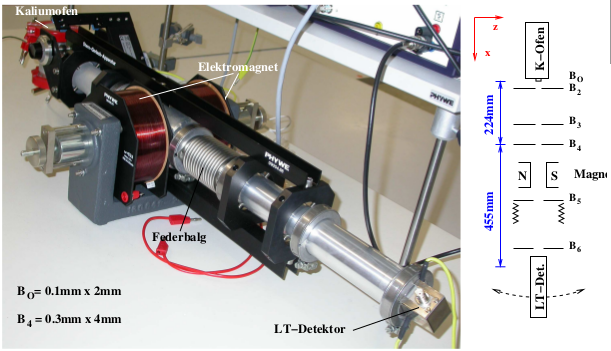
\includegraphics[width=\textwidth]{abbildungen/aufbau.png}
  \caption{Fotographie sowie schematische Darstellung der Versuchsapparatur.\cite{sample}}
  \label{fig:aufbau}
\end{figure}

\begin{figure}
  \centering
  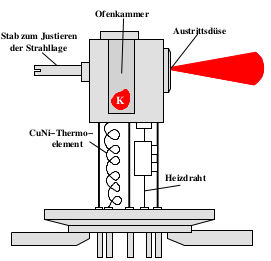
\includegraphics[width=0.5\textwidth]{abbildungen/ofen.png}
  \caption{Schematische Darstellung des Kaliumofens.\cite{sample}}
  \label{fig:ofen}
\end{figure}

\begin{figure}
  \centering
  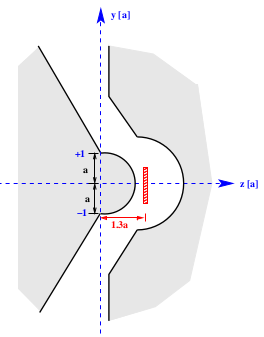
\includegraphics[width=0.5\textwidth]{abbildungen/magnet.png}
  \caption{Schematische Darstellung des verwendeten Magneten(Querschnitt).\cite{sample}}
  \label{fig:magnet}
\end{figure}
\FloatBarrier
\subsection{Messvorgang}
\label{subsec:d2}
Vor Messbeginn wird innerhalb der Versuchsapparatur ein Druck von $\SI{4.5e-6}{\milli\bar}$ hergestellt.
Der Ofen wird bei einem Heizsstrom von $\SI{0.6}{\ampere}$ auf eine Temperatur von $\SI{190}{\degreeCelsius}$
gebracht. Der Draht des Langmuir-Taylor-Detektors wird bei einer von ca. $\SI{9.5}{\volt}$ beheizt.\\
Der erste Messvorgang wird bei ausgeschaltetem Magneten durchgeführt. Es werden Wertepaare von gemessener
Spannung und Umdrehungen der Spindel aufgenommen.
Dabei werden nach Möglichkeit beide Maxima des (aufgespaltenen)
Strahls vermessen. Anschließend werden sieben weitere Messreihen bei eingeschaltetem Elektromageten
aufgenommen. Dabei werden die in Tabelle \ref{tab:messtabelle} angegebenen Werte für den
Strom $I$ beziehungsweise die Flussdichte $B$ verwendet.\\ \\
\begin{table}
  \centering
  \caption{Einstellungen des Elektromagneten für die verschiedenen Messreihen.}
  \label{tab:messtabelle}
  \begin{tabular}{c c c}
    \toprule
    $ \text{Nummer der Messreihe} $ & $ I \ / \ \si{\ampere} $ & $B \ / \ \si{\tesla}$\\
    \midrule
    1 & 0.16 & 0.11\\
    2 & 0.32 & 0.23\\
    3 & 0.41 & 0.30\\
    4 & 0.50 & 0.38\\
    5 & 0.60 & 0.45\\
    6 & 0.80 & 0.59\\
    7 & 0.90 & 0.65\\
    \bottomrule
  \end{tabular}
\end{table}
\\ \\Alle benötigten theoretischen Informationen zur Anfertigung der
Abschnitte \ref{sec:Theorie} und \ref{sec:Durchführung}
wurden der Versuchsanleitung \cite{sample} entnommen.
